\documentclass[11pt,a4paper,ngerman]{article}
\usepackage[bottom=2.5cm,top=2.5cm]{geometry} 
\usepackage{babel}
\usepackage[utf8]{inputenc} 
\usepackage[T1]{fontenc} 
\usepackage{ae} 
\usepackage{amssymb} 
\usepackage{amsmath} 
\usepackage{graphicx}
\usepackage{fancyhdr}
\usepackage{fancyref}
\usepackage{listings}
\usepackage{xcolor}
\usepackage{paralist}
\usepackage{subfigure}

%\usepackage[pdftex, bookmarks=false, pdfstartview={FitH}, linkbordercolor=white]{hyperref}
\usepackage{fancyhdr}
\pagestyle{fancy}
\fancyhead[C]{CoMa II}
\fancyhead[L]{Übung Nr. 6}
\fancyhead[R]{SoSe 2012}
\fancyfoot{}
\fancyfoot[L]{}
\fancyfoot[C]{\thepage / \pageref{LastPage}}
\renewcommand{\footrulewidth}{0.5pt}
\renewcommand{\headrulewidth}{0.5pt}
\setlength{\parindent}{0pt} 
\setlength{\headheight}{0pt}

\author{Tutor: Sebastian Scherer}
\date{}
\title{Max Wisniewski , Alexander Steen}

\begin{document}

\lstset{language=Pascal, basicstyle=\ttfamily\fontsize{10pt}{10pt}\selectfont\upshape, commentstyle=\rmfamily\itshape\small, keywordstyle=\rmfamily\bfseries, breaklines=true, frame=single, xleftmargin=3mm, xrightmargin=3mm, tabsize=2}

\maketitle
\thispagestyle{fancy}


%% ------------------------------------------------------
%%                     AUFGABE 1
%% ------------------------------------------------------

\section*{Aufgabe 1}

\begin{description}
\item[a)] Da $s_n(x)$ auf jedem Intervall $[x_i,x_{i+1}), 0 \leq i \leq n-2$ konstant gleich $f\left(\frac{x_{i} + x_{i+1}}{2}\right)$ ist (für das letzte Intervall analog als geschlossenes Intervall), können wir die Quadraturformel erhalten, in dem wir den Inhalt jedes Intervallrechtecks einzeln aufsummieren. Also ergibt sich die Formel

$$ \int_a^b s_n \, dx = h \cdot \sum_{i=0}^{n-1}{f\left( \frac{x_{i} + x_{i+1}}{2} \right)}$$
mit $h = \frac{b-a}{n}$ als konstante Breite der Streifen.

\item[b)] Testweise wurde $f = \sin$ gewählt und auf dem Intervall $[0,2 \pi]$ geplottet. Vergleichend wurde ebenfalls $s_{20}$ geplottet. 


\begin{figure}[ht]
\centering
	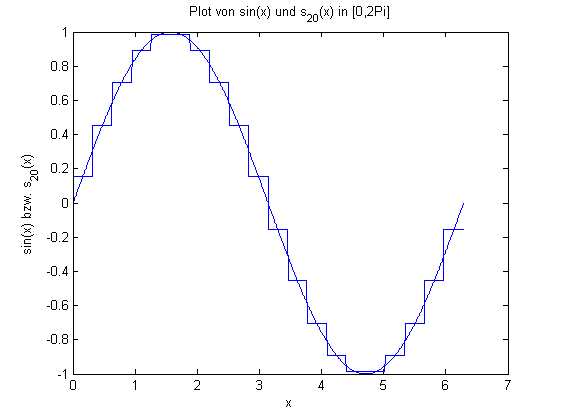
\includegraphics[scale=0.8]{quadneubeispiel}
\caption{Plot von $sin$ bzw. $s_{20}$.}
\end{figure}
\newpage
\item[c)] Die folgende Funktion berechnet numerisch das Integral nach obiger Defintion: \\

\begin{lstlisting}
function y = gauss(f, n, a, b)
% Diese Funktion berechnet die Integral
% von f von a bis b mittels
% Gauss-Quadratur und
% sog. Mittelpunktregel
% f Funktion
% n Anzahl der Stuetzstellen
% a, b Grenzen

% Breite des Gitters
h = (b-a)/n;
% Schritte im Intervall
xi = a:h:b;
% Berechne Funktionswerte an den geg. Stellen
for i = 1:n,
   fx(i) = f((xi(i)+xi(i+1))/2);
end
% Aufsummieren
y = h * sum(fx);
\end{lstlisting}

\item[d)] "[...] die Quadraturformeln heissen Gauss-Formeln bzw. man spricht von Gauss-Quadratur." (Wensch, Jörg: Computerorientiertes Rechnen Skript, Seite 38).
\end{description}




%% ------------------------------------------------------
%%                     AUFGABE 2
%% ------------------------------------------------------

\section*{Aufgabe 2}

\begin{description}
\item[a)] $\dot{x}(t) = 2x(t)$ \\
(i) Gewöhnlich: Es treten nur Ableitungen nach einer Variablen auf\\

(ii) Linear: Gilt, da für Lösungen $f,g$ gilt: $(\alpha f + \beta g)' = \alpha f' + \beta g' = \alpha 2f + \beta 2g = 2 (\alpha f + \alpha g)$. Damit sind alle Linearkombinationen von Lösungen wieder Lösungen. \\

(iii) 1. Ordnung:  Es treten nur Ableitung der 1. Ordnung auf. \\
$\Rightarrow$ Gewöhnliche, lineare Differentialgleichung 1. Ordnung.
\item[b)] $\dot{x}(t) = 4x(t)^2 + x(t)$ \\
Linearität nicht gegeben:  \\
Für Lösungen $f,g$ gilt: $(f + g)' = f' + g' = 4f^2 + f + 4g^2 + g = 4(f^2 + g^2) + (f+g)$. Da i.A. $(f+g)^2 \neq (f^2 + g^2)$, ist $(f+g)$ keine Lösung der Differentialgleichung.
\item[c)] $\ddot{x}(t) = \lambda x(t) +1$\\
Die Differentialgleichung ist nicht 1. Ordnung, da Ableitungen der 2. Ordnung auftreten.
\end{description}

\newpage
%% ------------------------------------------------------
%%                     AUFGABE 3
%% ------------------------------------------------------

\section*{Aufgabe 3}
Zu lösendes System von Differentialgleichungen:
$$
\begin{array}{lcr}
x' &=& y \\
y' &=& -y
\end{array}
$$

\textbf{Lösung}:\\
Wie aus dem Skript bekannt, lässt sich die Differentialgleichung $y' = -y$ durch $\alpha e^{-t}, \alpha \in \mathbb{R}$ lösen. Setzen wir den Anfangswert $y(0) = 1$ ein, ergibt sich für $\alpha$: $1 = y(0) = \alpha e^{0} = \alpha \Leftrightarrow \alpha = 1$. Also löst $y(t) = e^{-t}$ den unteren Teil des Gleichungssystems.

Suchen wir nun eine Funktion $x(t)$, mit $x'(t) = y(t) = e^{-t}$. Durch Integrieren erhalten wir als Lösung $x(t) = -e^{-t} + c, c \in \mathbb{R}$. Durch Einsetzen des Anfangswertes erhalten wir schließlich: $0 = x(0) = -e^{0} + c = -1+c \Leftrightarrow c = 1$.

Also ist die Lösung des Systems von Differentialgleichungen:
$$
\begin{array}{lcl}
x(t) &=& 1-e^{-t} \\
y(t) &=& e^{-t}
\end{array}
$$

\label{LastPage}

\end{document}
